\documentclass{article}

\usepackage[most]{tcolorbox}
\usepackage{mathtools}
\usepackage{physics}
\usepackage{graphicx}
\usepackage{float}


\usepackage[utf8]{inputenc}
\usepackage[a4paper,landscape, margin=0.1in]{geometry} % Controla los márgenes
\usepackage{titling}


\renewcommand{\maketitlehooka}{%
  \centering
  \vspace*{0.05cm} % Espacio vertical antes del título
}

\renewcommand{\maketitlehookd}{%
  \vspace*{2cm} % Espacio vertical después de la fecha
}

\newcommand{\caja}[3]{%
  \begin{tcolorbox}[colback=#1!5!white,colframe=#1!25!black,title=#2]
    #3
  \end{tcolorbox}%
}

\begin{document}

\begin{figure}[H]
  \begin{center}
    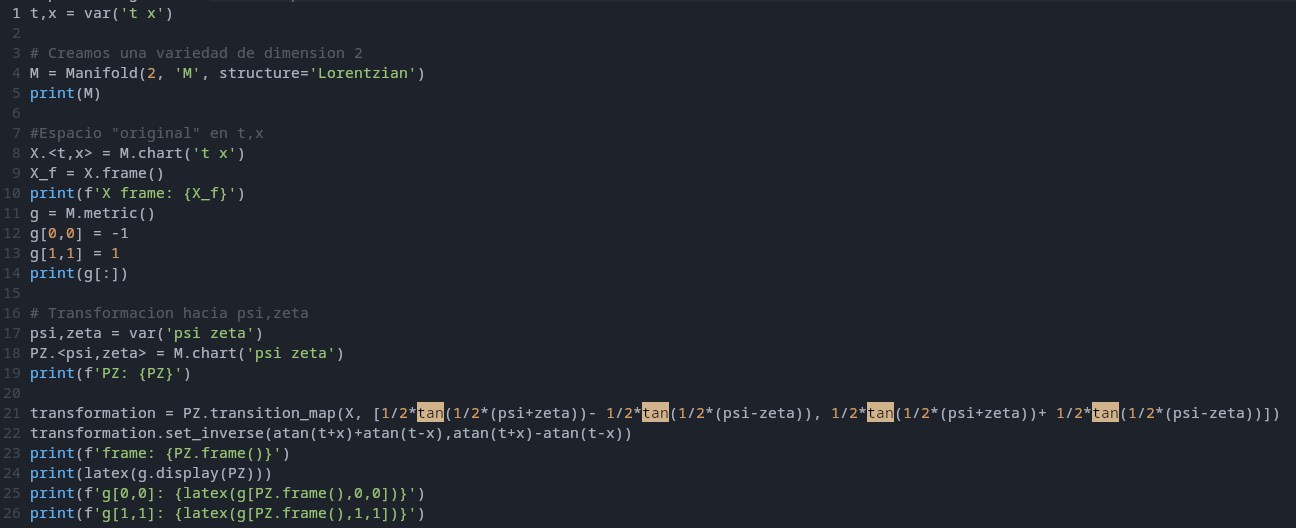
\includegraphics[width=0.95\textwidth]{codigo.png}
  \end{center}
\end{figure}

Se logró calcular la metrica pero la expresion es extremadamente larga y no se logró identificar el facto omega.

A continuacion dejo el resultado que se obtuvo para g en formato latex: 

\begin{gather*}
  g = \left( \frac{\cos\left(\frac{1}{2} \, \zeta\right)^{4} - 2 \, \cos\left(\frac{1}{2} \, \zeta\right)^{2} \sin\left(\frac{1}{2} \, \psi\right)^{2} + \sin\left(\frac{1}{2} \, \psi\right)^{4}}{4 \, {\left(\cos\left(\frac{1}{2} \, \psi\right)^{8} \cos\left(\frac{1}{2} \, \zeta\right)^{8} - 4 \, \cos\left(\frac{1}{2} \, \psi\right)^{6} \cos\left(\frac{1}{2} \, \zeta\right)^{6} \sin\left(\frac{1}{2} \, \psi\right)^{2} \sin\left(\frac{1}{2} \, \zeta\right)^{2} + 6 \, \cos\left(\frac{1}{2} \, \psi\right)^{4} \cos\left(\frac{1}{2} \, \zeta\right)^{4} \sin\left(\frac{1}{2} \, \psi\right)^{4} \sin\left(\frac{1}{2} \, \zeta\right)^{4} - 4 \, \cos\left(\frac{1}{2} \, \psi\right)^{2} \cos\left(\frac{1}{2} \, \zeta\right)^{2} \sin\left(\frac{1}{2} \, \psi\right)^{6} \sin\left(\frac{1}{2} \, \zeta\right)^{6} + \sin\left(\frac{1}{2} \, \psi\right)^{8} \sin\left(\frac{1}{2} \, \zeta\right)^{8}\right)}} \right) \mathrm{d} \psi\otimes \mathrm{d} \psi \\
  + \left( -\frac{\cos\left(\frac{1}{2} \, \zeta\right)^{4} - 2 \, \cos\left(\frac{1}{2} \, \zeta\right)^{2} \sin\left(\frac{1}{2} \, \psi\right)^{2} + \sin\left(\frac{1}{2} \, \psi\right)^{4}}{4 \, {\left(\cos\left(\frac{1}{2} \, \psi\right)^{8} \cos\left(\frac{1}{2} \, \zeta\right)^{8} - 4 \, \cos\left(\frac{1}{2} \, \psi\right)^{6} \cos\left(\frac{1}{2} \, \zeta\right)^{6} \sin\left(\frac{1}{2} \, \psi\right)^{2} \sin\left(\frac{1}{2} \, \zeta\right)^{2} + 6 \, \cos\left(\frac{1}{2} \, \psi\right)^{4} \cos\left(\frac{1}{2} \, \zeta\right)^{4} \sin\left(\frac{1}{2} \, \psi\right)^{4} \sin\left(\frac{1}{2} \, \zeta\right)^{4} - 4 \, \cos\left(\frac{1}{2} \, \psi\right)^{2} \cos\left(\frac{1}{2} \, \zeta\right)^{2} \sin\left(\frac{1}{2} \, \psi\right)^{6} \sin\left(\frac{1}{2} \, \zeta\right)^{6} + \sin\left(\frac{1}{2} \, \psi\right)^{8} \sin\left(\frac{1}{2} \, \zeta\right)^{8}\right)}} \right) \mathrm{d} \zeta\otimes \mathrm{d} \zeta\\
  g[0,0]: \frac{1}{4 \, {\left(4 \, {\left(4 \, \cos\left(\frac{1}{2} \, \arctan\left(-t + x\right)\right)^{4} - 4 \, \cos\left(\frac{1}{2} \, \arctan\left(-t + x\right)\right)^{2} + 1\right)} \cos\left(\frac{1}{2} \, \arctan\left(t + x\right)\right)^{4} + 4 \, \cos\left(\frac{1}{2} \, \arctan\left(-t + x\right)\right)^{4} - 4 \, {\left(4 \, \cos\left(\frac{1}{2} \, \arctan\left(-t + x\right)\right)^{4} - 4 \, \cos\left(\frac{1}{2} \, \arctan\left(-t + x\right)\right)^{2} + 1\right)} \cos\left(\frac{1}{2} \, \arctan\left(t + x\right)\right)^{2} - 4 \, \cos\left(\frac{1}{2} \, \arctan\left(-t + x\right)\right)^{2} + 1\right)}}\\
  g[1,1]: -\frac{1}{4 \, {\left(4 \, {\left(4 \, \cos\left(\frac{1}{2} \, \arctan\left(-t + x\right)\right)^{4} - 4 \, \cos\left(\frac{1}{2} \, \arctan\left(-t + x\right)\right)^{2} + 1\right)} \cos\left(\frac{1}{2} \, \arctan\left(t + x\right)\right)^{4} + 4 \, \cos\left(\frac{1}{2} \, \arctan\left(-t + x\right)\right)^{4} - 4 \, {\left(4 \, \cos\left(\frac{1}{2} \, \arctan\left(-t + x\right)\right)^{4} - 4 \, \cos\left(\frac{1}{2} \, \arctan\left(-t + x\right)\right)^{2} + 1\right)} \cos\left(\frac{1}{2} \, \arctan\left(t + x\right)\right)^{2} - 4 \, \cos\left(\frac{1}{2} \, \arctan\left(-t + x\right)\right)^{2} + 1\right)}}
\end{gather*}


\end{document}
